% generated by Docutils <http://docutils.sourceforge.net/>
\documentclass[a4paper,english]{article}
\usepackage{fixltx2e} % LaTeX patches, \textsubscript
\usepackage{cmap} % fix search and cut-and-paste in PDF
\usepackage{babel}
\usepackage[T1]{fontenc}
\usepackage[latin1]{inputenc}
\usepackage{ifthen}
\usepackage{graphicx}
\usepackage{multirow}
\usepackage{longtable}
\usepackage{array}
\setlength{\extrarowheight}{2pt}
\newlength{\DUtablewidth} % internal use in tables

%%% User specified packages and stylesheets

 \usepackage[default,osfigures,scale=0.95]{opensans}
 \usepackage{xspace}
 \usepackage{fancyhdr}
 \usepackage{graphicx}
 \usepackage{enumitem}
 \usepackage[sf,bf]{titlesec}
 \usepackage{titletoc}
 \usepackage[paper=a4paper,headheight=30pt,tmargin=1.5in,bmargin=1in]{geometry}
%\usepackage{layouts}

 \renewlist{itemize}{itemize}{9}
 \setlist[itemize]{label=\textbullet}

% The LaTeX Companion -- p. 204.
% Miniature display of the page layout.
%\newcommand{\showpage}{%
%  \setlayoutscale{0.65}\setlabelfont{\tiny}%
%  \printheadingsfalse\printparametersfalse%
%  \currentpage\pagedesign%
%}

 \titlecontents{section}[0pc]
   {\sffamily\bfseries}                                   % above code.
   {\contentslabel{1pc}}                                  % numbered entry format.
   {}                                                     % numberless entry format.
   {\titlerule*[8pt]{.}\textsc{\textbf{{\contentspage}}}} % page format.
 \titlecontents{subsection}[0pc]
   {\sffamily}                                            % above code.
   {\contentslabel{2pc}}                                  % numbered entry format.
   {}                                                     % numberless entry format.
   {\titlerule*[8pt]{.}\textsc{\textbf{{\contentspage}}}} % page format.
 \titlecontents{subsubsection}[1pc]
   {\sffamily}                                            % above code.
   {\contentslabel{2pc}}                                  % numbered entry format.
   {}                                                     % numberless entry format.
   {\titlerule*[8pt]{.}\textsc{\textbf{{\contentspage}}}} % page format.

 \newcommand{\key}[1]{\raisebox{-0.5\baselineskip}{\rule{0pt}{1.5\baselineskip}}\fbox{\textsf{#1}}}

 \newcommand{\DUroleul}[1]{\underline{#1}\xspace}
 \newcommand{\DUrolesc}[1]{\textsc{#1}\xspace}
 \newcommand{\DUrolecb}[1]{\textbf{\texttt{#1}}\xspace}
 \newcommand{\DUrolefboxtt}[1]{\fbox{\texttt{#1}}\xspace}

 \newcommand{\DUtitlenote}[1]{\noindent\textbf{#1}\smallskip}

 \newcommand{\DUadmonitionnote}[1]{%
   \begin{center}
     \sffamily
     \begin{array}[t]{m{1cm}!{\vrule width 1pt}m{.90\textwidth}}
       \raisebox{0.0cm}{
\includegraphics[scale=0.5]{./images/clipboard.eps}} &
       \begin{minipage}[t]{.85\textwidth} #1
       \end{minipage} \\
     \end{array}
   \end{center}
 }

 \newcommand{\DUtitleerror}[1]{\noindent\textbf{\color{red}#1}\smallskip}

 \newcommand{\DUadmonitionerror}[1]{%
   \begin{center}
     \sffamily
     \begin{array}[t]{m{1cm}!{\vrule width 1pt}m{.90\textwidth}}
       \raisebox{0.0cm}{
\includegraphics[scale=0.5]{./images/i-core.eps}} &
       \begin{minipage}[t]{.85\textwidth} #1
       \end{minipage} \\
     \end{array}
   \end{center}
 }

 \newcommand{\UPMC}               {\textsc{upmc}\xspace}
 \newcommand{\LIP}                {\textsc{lip6}\xspace}
 \newcommand{\SoC}                {\textsc{S}o\textsc{C}\xspace}

 \renewcommand{\headrulewidth}{0.2mm}
 \renewcommand{\footrulewidth}{0.2mm}
 \renewcommand{\sectionmark}[1]{\markboth{\thesection\ #1}{\thesection\ #1}}
 \renewcommand{\subsectionmark}[1]{}
 \lhead[]{Documentation \SoC}
 \rhead[]{March 2014}
 \lfoot[]{\UPMC/\LIP/\SoC}
 \rfoot[]{\thepage}
 \cfoot[]{}

 \pagestyle{fancy}


%%% Fallback definitions for Docutils-specific commands

% providelength (provide a length variable and set default, if it is new)
\providecommand*{\DUprovidelength}[2]{
  \ifthenelse{\isundefined{#1}}{\newlength{#1}\setlength{#1}{#2}}{}
}

% admonition (specially marked topic)
\providecommand{\DUadmonition}[2][class-arg]{%
  % try \DUadmonition#1{#2}:
  \ifcsname DUadmonition#1\endcsname%
    \csname DUadmonition#1\endcsname{#2}%
  \else
    \begin{center}
      \fbox{\parbox{0.9\textwidth}{#2}}
    \end{center}
  \fi
}

% inline markup (custom roles)
% \DUrole{#1}{#2} tries \DUrole#1{#2}
\providecommand*{\DUrole}[2]{%
  \ifcsname DUrole#1\endcsname%
    \csname DUrole#1\endcsname{#2}%
  \else% backwards compatibility: try \docutilsrole#1{#2}
    \ifcsname docutilsrole#1\endcsname%
      \csname docutilsrole#1\endcsname{#2}%
    \else%
      #2%
    \fi%
  \fi%
}

% lineblock environment
\DUprovidelength{\DUlineblockindent}{2.5em}
\ifthenelse{\isundefined{\DUlineblock}}{
  \newenvironment{DUlineblock}[1]{%
    \list{}{\setlength{\partopsep}{\parskip}
            \addtolength{\partopsep}{\baselineskip}
            \setlength{\topsep}{0pt}
            \setlength{\itemsep}{0.15\baselineskip}
            \setlength{\parsep}{0pt}
            \setlength{\leftmargin}{#1}}
    \raggedright
  }
  {\endlist}
}{}

% title for topics, admonitions and sidebar
\providecommand*{\DUtitle}[2][class-arg]{%
  % call \DUtitle#1{#2} if it exists:
  \ifcsname DUtitle#1\endcsname%
    \csname DUtitle#1\endcsname{#2}%
  \else
    \smallskip\noindent\textbf{#2}\smallskip%
  \fi
}

% titlereference role
\providecommand*{\DUroletitlereference}[1]{\textsl{#1}}

% hyperlinks:
\ifthenelse{\isundefined{\hypersetup}}{
  \usepackage[colorlinks=true,linkcolor=blue,urlcolor=blue]{hyperref}
}{}
\hypersetup{
  pdftitle={Coriolis User's Guide},
}

%%% Body
\begin{document}

% Document title
\title{Coriolis User's Guide%
  \phantomsection%
  \label{coriolis-user-s-guide}}
\author{}
\date{}
\maketitle

% -*- Mode: rst -*-

% -*- Mode: rst -*-

% For LaTeX/PDF backend.

% Stand-alone images.

% Direct LaTeX commands encapsulation.

% -*- Mode: rst -*-

% Acronyms & names.

% URLs

% Standard CAO/VLSI Concepts.

% MBK Concepts

% Hurricane Concepts.

\phantomsection\label{contents}
\pdfbookmark[1]{Contents}{contents}
\tableofcontents


\DUrole{raw-latex}{\newpage}


%___________________________________________________________________________

\section*{Credits \& License%
  \phantomsection%
  \addcontentsline{toc}{section}{Credits \& License}%
  \label{credits-license}%
}
\begin{center}\begin{minipage}[t]{.8\textwidth}
  \noindent\DUrole{sc}{Hurricane} \dotfill R�my       \DUrole{sc}{Escassut}  \&
                                           Christian  \DUrole{Masson}        \\
  \noindent\DUrole{sc}{Mauka}     \dotfill Christophe \DUrole{sc}{Alexandre} \\
  \noindent\DUrole{sc}{Stratus}   \dotfill Sophie     \DUrole{sc}{Belloeil}  \\
  \noindent\DUrole{sc}{Knik}      \dotfill Damien     \DUrole{sc}{Dupuis}    \\
  \noindent\DUrole{sc}{Kite},
           \DUrole{sc}{Unicorn}   \dotfill Jean-Paul \DUrole{sc}{Chaput}     \\
\end{minipage}\end{center}
\DUrole{raw-latex}{\medskip}

The \DUrole{sc}{Hurricane} data-base is copyright� \DUrole{sc}{Bull} 2000-2012 and is
released under the terms of the \DUrole{sc}{lgpl} license. All other tools are
copyright� \DUrole{sc}{upmc} 2008-2012 and released under the \DUrole{sc}{gpl}
license.

The \DUrole{sc}{Knik} router makes use of the \DUrole{sc}{Flute} software, which is
copyright� Chris C. N. \DUrole{sc}{Chu} from the Iowa State University
(\href{http://home.eng.iastate.edu/~cnchu/}{http://home.eng.iastate.edu/\textasciitilde{}cnchu/}).

\DUrole{raw-latex}{\newpage}


%___________________________________________________________________________

\section*{Release Notes%
  \phantomsection%
  \addcontentsline{toc}{section}{Release Notes}%
  \label{release-notes}%
}


%___________________________________________________________________________

\subsection*{Release 1.0.1475%
  \phantomsection%
  \addcontentsline{toc}{subsection}{Release 1.0.1475}%
  \label{release-1-0-1475}%
}

This is the first preliminary release of the \DUrole{sc}{Coriolis 2} framework.

This release mainly ships the global router \DUrole{sc}{Knik} and the detailed router
\DUrole{sc}{Kite}. Together they aim to replace the \DUrole{sc}{Alliance} \DUrole{sc}{Nero} router.
Unlike \DUrole{sc}{Nero}, \DUrole{sc}{Kite} is based on an innovating routing modeling and ad-hoc
algorithm. Although it is released under \DUrole{sc}{gpl} license, the source code
will be avalaible later.
\DUrole{raw-latex}{\medskip}

\DUrole{raw-latex}{\noindent} Contents of this release:
\newcounter{listcnt0}
\begin{list}{\arabic{listcnt0}.}
{
\usecounter{listcnt0}
\setlength{\rightmargin}{\leftmargin}
}

\item A graphical user interface (viewer only).

\item The \DUrole{sc}{Knik} global router.

\item The \DUrole{sc}{Kite} detailed router.
\end{list}

\DUrole{raw-latex}{\noindent} Supported input/output formats:
%
\begin{itemize}

\item \DUrole{sc}{Alliance} \DUrole{cb}{vst} (netlist) \& \DUrole{cb}{ap} (physical) formats.

\item Even if there are some references to the \DUrole{sc}{Cadence} \DUrole{sc}{lefdef} format, its
support is not included because it depends on a library only available
to \DUrole{sc}{Si2} affiliated members.

\end{itemize}


%___________________________________________________________________________

\subsection*{Release 1.0.1963%
  \phantomsection%
  \addcontentsline{toc}{subsection}{Release 1.0.1963}%
  \label{release-1-0-1963}%
}

Release 1963 is alpha. All the tools from \DUrole{sc}{Coriolis 1} have been ported into
this release.

\DUrole{raw-latex}{\noindent} Contents of this release:
\setcounter{listcnt0}{0}
\begin{list}{\arabic{listcnt0}.}
{
\usecounter{listcnt0}
\setlength{\rightmargin}{\leftmargin}
}

\item The \DUrole{sc}{Stratus} netlist capture language (\DUrole{sc}{GenLib} replacement).

\item The \DUrole{sc}{Mauka} placer (still contains bugs).

\item A graphical user interface (viewer only).

\item The \DUrole{sc}{Knik} global router.

\item The \DUrole{sc}{Kite} detailed router.

\item Partially implemented python support for configuration files
(alternative to \DUrole{sc}{xml}).

\item A documentation (imcomplete/obsoleted in \DUrole{sc}{Hurricane}'s case).
\end{list}


%___________________________________________________________________________

\subsection*{Release 1.0.xxxx%
  \phantomsection%
  \addcontentsline{toc}{subsection}{Release 1.0.xxxx}%
  \label{release-1-0-xxxx}%
}

Release \DUroletitlereference{xxxx} is RC1.

\DUrole{raw-latex}{\noindent} Changes of this release:
\setcounter{listcnt0}{0}
\begin{list}{\arabic{listcnt0}.}
{
\usecounter{listcnt0}
\setlength{\rightmargin}{\leftmargin}
}

\item The \DUrole{sc}{Hurricane} documentation is now accurate. Documentation
for the Cell viewer and \DUrole{sc}{CRLcore} has been added.

\item More extensive Python support for all the components of
\DUrole{sc}{Coriolis}.

\item Configuration is now completly migrated under Python.
\DUrole{sc}{xml} loaders can still be useds for compatibilty.

\item The \DUrole{cb}{cgt} main has been rewritten in Python.
\end{list}

\DUrole{raw-latex}{\newpage}


%___________________________________________________________________________

\section*{Installation%
  \phantomsection%
  \addcontentsline{toc}{section}{Installation}%
  \label{installation}%
}

Binary packages avalaible:

\leavevmode
\setlength{\DUtablewidth}{\linewidth}
\begin{longtable}[c]{|p{0.284\DUtablewidth}|p{0.551\DUtablewidth}|}
\hline
\textbf{%
Distribution
} & \textbf{%
Package
} \\
\hline
\endfirsthead
\hline
\textbf{%
Distribution
} & \textbf{%
Package
} \\
\hline
\endhead
\multicolumn{2}{c}{\hfill ... continued on next page} \\
\endfoot
\endlastfoot

\DUrole{sc}{Scientific Linux} 6
 & 
\begin{DUlineblock}{0em}
\item[] \href{http://asim.lip6.fr/pub/coriolis/2.0/coriolis2-1.0.xxxx-1.slsoc6.i686.rpm}{coriolis2-1.0.xxxx-1.slsoc6.i686.rpm}
\item[] \href{http://asim.lip6.fr/pub/coriolis/2.0/coriolis2-1.0.xxxx-1.slsoc6.x86_64.rpm}{coriolis2-1.0.xxxx-1.slsoc6.x86\_64.rpm}
\end{DUlineblock}
 \\
\hline

\DUrole{sc}{Fedora} 16
 & 
\begin{DUlineblock}{0em}
\item[] \href{http://asim.lip6.fr/pub/coriolis/2.0/coriolis2-1.0.xxxx-1.fc16.i686.rpm}{coriolis2-1.0.xxxx-1.fc16.i686.rpm}
\item[] \href{http://asim.lip6.fr/pub/coriolis/2.0/coriolis2-1.0.xxxx-1.fc16.x86_64.rpm}{coriolis2-1.0.xxxx-1.fc16.x86\_64.rpm}
\end{DUlineblock}
 \\
\hline

\DUrole{sc}{Ubuntu} 10.04 LTS
 & 
\begin{DUlineblock}{0em}
\item[] \href{http://asim.lip6.fr/pub/coriolis/2.0/Ubuntu/10.04/coriolis2_1.0-xxxx-1_i386.rpm}{coriolis2\_1.0-xxxx-1\_.i386.rpm (10.04)}
\item[] \href{http://asim.lip6.fr/pub/coriolis/2.0/Ubuntu/10.04/coriolis2_1.0-xxxx-1_i386.rpm}{coriolis2\_1.0-xxxx-1\_.amd64.rpm (10.04)}
\end{DUlineblock}
 \\
\hline

\DUrole{sc}{Ubuntu} 12.04 LTS
 & 
\begin{DUlineblock}{0em}
\item[] \href{http://asim.lip6.fr/pub/coriolis/2.0/Ubuntu/12.04/coriolis2_1.0-xxxx-1_i386.rpm}{coriolis2\_1.0-xxxx-1\_.i386.rpm (12.04)}
\item[] \href{http://asim.lip6.fr/pub/coriolis/2.0/Ubuntu/12.04/coriolis2_1.0-xxxx-1_i386.rpm}{coriolis2\_1.0-xxxx-1\_.amd64.rpm (12.04)}
\end{DUlineblock}
 \\
\hline
\end{longtable}

If you are installing from source, you should go to section \hyperref[installation-from-sources]{Installation From Sources}.

\DUrole{raw-latex}{\newpage}


%___________________________________________________________________________

\section*{Coriolis Configuration \& Initialisation%
  \phantomsection%
  \addcontentsline{toc}{section}{Coriolis Configuration \& Initialisation}%
  \label{coriolis-configuration-initialisation}%
}

All configuration \& initialization files are Python scripts, despite their
\DUrole{cb}{.conf} extention. From a syntactic point of view, there is no difference
between the system-wide configuration files and the user's configuration,
they may use the same Python helpers.
\DUrole{raw-latex}{\medskip}

\DUrole{raw-latex}{\noindent}
The initialization process is done by executing, in order, the following
file(s):

\leavevmode
\setlength{\DUtablewidth}{\linewidth}
\begin{longtable}[c]{|p{0.088\DUtablewidth}|p{0.367\DUtablewidth}|p{0.491\DUtablewidth}|}
\hline
\textbf{%
Order
} & \textbf{%
Meaning
} & \textbf{%
File
} \\
\hline
\endfirsthead
\hline
\textbf{%
Order
} & \textbf{%
Meaning
} & \textbf{%
File
} \\
\hline
\endhead
\multicolumn{3}{c}{\hfill ... continued on next page} \\
\endfoot
\endlastfoot

\textbf{1}
 & 
The system initialization
 & 
\DUrole{cb}{/etc/coriolis2/coriolisInit.py}
 \\
\hline

\textbf{2}
 & 
The user's global initialization
 & 
\DUrole{cb}{\$\{HOME\}/.coriolis2.conf}
 \\
\hline

\textbf{3}
 & 
The user's local initialization
 & 
\DUrole{cb}{<CWD>/.coriolis2.conf}
 \\
\hline
\end{longtable}

\DUadmonition[note]{
\DUtitle[note]{Note}

\emph{The loading policy is not hard-coded.} It is implemented
at Python level in \DUrole{cb}{coriolisInit.py}, and thus may be easyly be
amended to whatever site policy.

The truly mandatory requirement is the existence of \DUrole{cb}{coriolisInit.py}
which \emph{must} contain a \DUrole{cb}{coriolisConfigure()} function with no argument.
}


%___________________________________________________________________________

\subsection*{Configuration Helpers%
  \phantomsection%
  \addcontentsline{toc}{subsection}{Configuration Helpers}%
  \label{configuration-helpers}%
}

To ease the writing of configuration files, a set of small helpers
is available. They allow to setup the configuration parameters through
simple assembly of tuples.


%___________________________________________________________________________

\subsubsection*{\DUrole{sc}{Alliance} Helper%
  \phantomsection%
  \addcontentsline{toc}{subsubsection}{Alliance Helper}%
  \label{alliance-helper}%
}

The configuration file must provide a \DUrole{cb}{allianceConfig} tuple of
the form:
%
\begin{quote}{\ttfamily \raggedright \noindent
cellsTop~=~'/soc/alliance/cells/'\\
~\\
allianceConfig~=~\textbackslash{}\\
~~~~(~(~'SYMBOLIC\_TECHNOLOGY',~helpers.sysConfDir+'/technology.symbolic.xml'~~~)\\
~~~~,~(~'REAL\_TECHNOLOGY'~~~~,~helpers.sysConfDir+'/technology.cmos130.s2r.xml')\\
~~~~,~(~'DISPLAY'~~~~~~~~~~~~,~helpers.sysConfDir+'/display.xml'~~~~~~~~~~~~~~~)\\
~~~~,~(~'CATALOG'~~~~~~~~~~~~,~'CATAL')\\
~~~~,~(~'WORKING\_LIBRARY'~~~~,~'.')\\
~~~~,~(~'SYSTEM\_LIBRARY'~~~~~,~(~(cellsTop+'sxlib'~~~,~Environment.Append)\\
~~~~~~~~~~~~~~~~~~~~~~~~~~~~~~~,~(cellsTop+'dp\_sxlib',~Environment.Append)\\
~~~~~~~~~~~~~~~~~~~~~~~~~~~~~~~,~(cellsTop+'ramlib'~~,~Environment.Append)\\
~~~~~~~~~~~~~~~~~~~~~~~~~~~~~~~,~(cellsTop+'romlib'~~,~Environment.Append)\\
~~~~~~~~~~~~~~~~~~~~~~~~~~~~~~~,~(cellsTop+'rflib'~~~,~Environment.Append)\\
~~~~~~~~~~~~~~~~~~~~~~~~~~~~~~~,~(cellsTop+'rf2lib'~~,~Environment.Append)\\
~~~~~~~~~~~~~~~~~~~~~~~~~~~~~~~,~(cellsTop+'pxlib'~~~,~Environment.Append)~)~)\\
~~~~,~(~'SCALE\_X'~~~~~~~~~~~~,~100)\\
~~~~,~(~'IN\_LO'~~~~~~~~~~~~~~,~'vst')\\
~~~~,~(~'IN\_PH'~~~~~~~~~~~~~~,~'ap')\\
~~~~,~(~'OUT\_LO'~~~~~~~~~~~~~,~'vst')\\
~~~~,~(~'OUT\_PH'~~~~~~~~~~~~~,~'ap')\\
~~~~,~(~'POWER'~~~~~~~~~~~~~~,~'vdd')\\
~~~~,~(~'GROUND'~~~~~~~~~~~~~,~'vss')\\
~~~~,~(~'CLOCK'~~~~~~~~~~~~~~,~'\textasciicircum{}ck.*')\\
~~~~,~(~'BLOCKAGE'~~~~~~~~~~~,~'\textasciicircum{}blockageNet*')\\
~~~~)
}
\end{quote}

\DUrole{raw-latex}{\noindent} The example above shows the system configuration file, with all the
available settings. Some important remarks about thoses settings:
%
\begin{itemize}

\item In it's configuration file, the user do not need to redefine all the settings,
just the one he wants to change. In most of the cases, the \texttt{SYSTEM\_LIBRARY},
the \texttt{WORKING\_LIBRARY} and the special net names (at this point there is not
much alternatives for the others settings).

\item \texttt{SYSTEM\_LIBRARY} setting: Setting up the library search path.
Each library entry in the tuple will be added to the search path according
to the second parameter:
%
\begin{itemize}

\item \DUrole{cb}{Environment::Append}:  append to the search path.

\item \DUrole{cb}{Environment::Prepend}: insert in head of the search path.

\item \DUrole{cb}{Environment::Replace}: look for a library of the same name and replace
it, whithout changing the search path order. If no library of that name
already exists, it is appended.

\end{itemize}

A library is identified by it's name, this name is the last component of the
path name. For instance: \texttt{/soc/alliance/sxlib} will be named \texttt{sxlib}.
Implementing the \DUrole{sc}{Alliance} specification, when looking for a \emph{Cell} \texttt{name},
the system will browse sequentially trought the library list and returns
the first \emph{Cell} whose name match.

\item For \texttt{POWER}, \texttt{GROUND}, \texttt{CLOCK} and \texttt{BLOCKAGE} net names, a regular
expression (\DUrole{sc}{gnu} regexp) is expected.

\item The \texttt{helpers.sysConfDir} variable is supplied by the helpers, it is the
directory in which the system-wide configuration files are locateds.
For a standard installation it would be: \texttt{/soc/coriolis2}.

\item Trick and naming convention about \texttt{SYMBOLIC\_TECHNOLOGY}, \texttt{REAL\_TECHNOLOGY}
and \texttt{DISPLAY}. In the previous releases, thoses files where to read by
\DUrole{sc}{xml} parsers, and still do if you triggers the \DUrole{sc}{xml} compatibility mode.
But now, they have Python conterparts. In the configuration files, you
still have to name them as \DUrole{sc}{xml} files, the Python file name will be
deduced from this one with thoses two translation rules:
\setcounter{listcnt0}{0}
\begin{list}{\arabic{listcnt0}.}
{
\usecounter{listcnt0}
\setlength{\rightmargin}{\leftmargin}
}

\item In the filename, all dots, except for the last (the file extention),
are replaced by underscores.

\item The \texttt{.xml} extention is substituted by a \texttt{.conf}.
\end{list}

For the symbolic technology, it would give:
%
\begin{quote}{\ttfamily \raggedright \noindent
/soc/coriolis2/technology.symbolic.xml\\
~~~~~~~~~~~~~~~~~~~~~~~-{}->~/soc/coriolis2/technology\_symbolic.conf
}
\end{quote}

\end{itemize}

A typical user's configuration file would be:
%
\begin{quote}{\ttfamily \raggedright \noindent
import~os\\
~\\
homeDir~=~os.getenv('HOME')\\
~\\
allianceConfig~=~\textbackslash{}\\
~~~~(~('WORKING\_LIBRARY'~~~~,~homeDir+'/worklib')\\
~~~~,~('SYSTEM\_LIBRARY'~~~~~,~(~(homeDir+'/mylib',~Environment.Append)~)~)\\
~~~~,~('POWER'~~~~~~~~~~~~~~,~'vdd.*')\\
~~~~,~('GROUND'~~~~~~~~~~~~~,~'vss.*')\\
~~~~)
}
\end{quote}


%___________________________________________________________________________

\subsubsection*{Tools Configuration Helpers%
  \phantomsection%
  \addcontentsline{toc}{subsubsection}{Tools Configuration Helpers}%
  \label{tools-configuration-helpers}%
}

All the tools uses the same helper to load their configuration (a.k.a.
\emph{Configuration Helper}). Currently the following configuration system-wide
configuration files are defined:
%
\begin{itemize}

\item \DUrole{cb}{misc.conf}: commons settings or not belonging specifically to a tool.

\item \DUrole{cb}{nimbus.conf}: for the \DUrole{sc}{Nimbus} tool.

\item \DUrole{cb}{hMetis.conf}: for the \DUrole{sc}{hMetis} wrapper.

\item \DUrole{cb}{mauka.conf}: for the \DUrole{sc}{Mauka} tool.

\item \DUrole{cb}{kite.conf}: for the \DUrole{sc}{Kite} tool.

\item \DUrole{cb}{stratus1.conf}: for the \DUrole{sc}{Stratus1} tool.

\end{itemize}

Here is the contents of \DUrole{cb}{mauka.conf}:
%
\begin{quote}{\ttfamily \raggedright \noindent
\#~Mauka~parameters.\\
parametersTable~=~\textbackslash{}\\
~~~~(~('mauka.annealingBinMult'~,~TypePercentage,~5~~~~~~)\\
~~~~,~('mauka.annealingNetMult'~,~TypePercentage,~90~~~~~)\\
~~~~,~('mauka.annealingRowMult'~,~TypePercentage,~5~~~~~~)\\
~~~~,~('mauka.ignorePins'~~~~~~~,~TypeBool~~~~~~,~False~~)\\
~~~~,~('mauka.insertFeeds'~~~~~~,~TypeBool~~~~~~,~True~~~)\\
~~~~,~('mauka.plotBins'~~~~~~~~~,~TypeBool~~~~~~,~True~~~)\\
~~~~,~('mauka.searchRatio'~~~~~~,~TypePercentage,~50~~~~~)\\
~~~~,~('mauka.standardAnnealing',~TypeBool~~~~~~,~False~~)\\
~~~~)\\
~\\
layoutTable~=~\textbackslash{}\\
~~~~(~(TypeTab~~~,~'Mauka',~'mauka')\\
~~~~\#~Mauka~part.\\
~~~~,~(TypeOption,~"mauka.standardAnnealing",~"Standart~Annealing"~~~~,~0~)\\
~~~~,~(TypeOption,~"mauka.ignorePins"~~~~~~~,~"Ignore~Pins"~~~~~~~~~~~,~0~)\\
~~~~,~(TypeOption,~"mauka.plotBins"~~~~~~~~~,~"Plot~Bins"~~~~~~~~~~~~~,~0~)\\
~~~~,~(TypeOption,~"mauka.insertFeeds"~~~~~~,~"Insert~Feeds"~~~~~~~~~~,~0~)\\
~~~~,~(TypeOption,~"mauka.searchRatio"~~~~~~,~"Search~Ratio~(\%)"~~~~~~,~1~)\\
~~~~,~(TypeOption,~"mauka.annealingNetMult"~,~"Annealing~Net~Mult~(\%)",~1~)\\
~~~~,~(TypeOption,~"mauka.annealingBinMult"~,~"Annealing~Bin~Mult~(\%)",~1~)\\
~~~~,~(TypeOption,~"mauka.annealingRowMult"~,~"Annealing~Row~Mult~(\%)",~1~)\\
~~~~,~(TypeRule~~,)\\
~~~~)
}
\end{quote}

Taxonomy of the file:
%
\begin{itemize}

\item It must contains, at least, the two tables:
%
\begin{itemize}

\item \texttt{parametersTable}, defines \& initialise the configuration variables.

\item \texttt{layoutTables}, defines how the various parameters will be displayed
in the configuration window

\end{itemize}

\item The \texttt{parametersTable}, is a tuple (list) of tuples. Each entry in the list
describe a configuration parameter. In it's simplest form, it's a quadruplet
\DUrole{cb}{(TypeOption, 'paramId', ParameterType, DefaultValue)} with:
\setcounter{listcnt0}{0}
\begin{list}{\arabic{listcnt0}.}
{
\usecounter{listcnt0}
\setlength{\rightmargin}{\leftmargin}
}

\item \texttt{TypeOption}, tells that this tuple describe a parameter.

\item \texttt{paramId}, the identifier of the parameter. Identifiers are defined
by the tools. The list of parameters is detailed in each tool section.

\item \texttt{ParameterType}, the kind of parameter. Could be:
%
\begin{itemize}

\item \texttt{TypeBool}, boolean.

\item \texttt{TypeInt}, signed integer.

\item \texttt{TypeEnumerate}, enumerated type, needs extra entry.

\item \texttt{TypePercentage}, percentage, expressed between 0 and 100.

\item \texttt{TypeDouble}, float.

\item \texttt{TypeString}, character string.

\end{itemize}

\item \texttt{DefaultValue}, the default value for that parameter.
\end{list}

\end{itemize}


%___________________________________________________________________________

\section*{CGT - The Graphical Interface%
  \phantomsection%
  \addcontentsline{toc}{section}{CGT - The Graphical Interface}%
  \label{cgt-the-graphical-interface}%
}

The \DUrole{sc}{Coriolis} graphical interface is split up into two windows.
%
\begin{itemize}

\item The \textbf{Viewer}, with the following features:
%
\begin{itemize}

\item Basic load/save capabilities.

\item Display the current working cell. Could be empty if the design
is not yet placed.

\item Execute Stratus Scripts.

\item Menu to run the tools (placement, routage).

\end{itemize}

\end{itemize}

Features are detailed in \hyperref[viewer-tools]{Viewer \& Tools}.

\DUrole{raw-latex}{\begin{center}\fbox{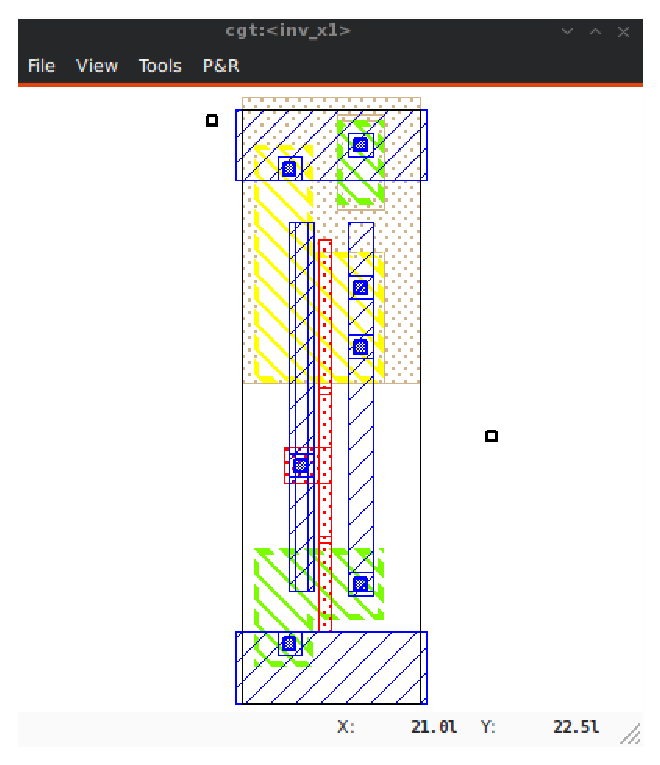
\includegraphics[width=.7\textwidth]{./images/Viewer-1.eps}}\end{center}}
%
\begin{itemize}

\item The \textbf{Controller}, which allows:
%
\begin{itemize}

\item Tweak what is displayer by the \emph{Viewer}. Through the \emph{Look},
\emph{Filter} and \emph{Layers\&Gos} tabs.

\item Browse the \emph{netlist} with eponym tab.

\item Show the list of selected objects (if any) with \emph{selection}

\item Walk through the Database, the Cell or the Selection with \emph{Inspector}.
This is an advanced feature, reserved for experimented users.

\item The tab \emph{Settings} which give access to all the settings.
They are closely related to Configuration \& Initialisation.

\end{itemize}

\end{itemize}

\DUrole{raw-latex}{\begin{center}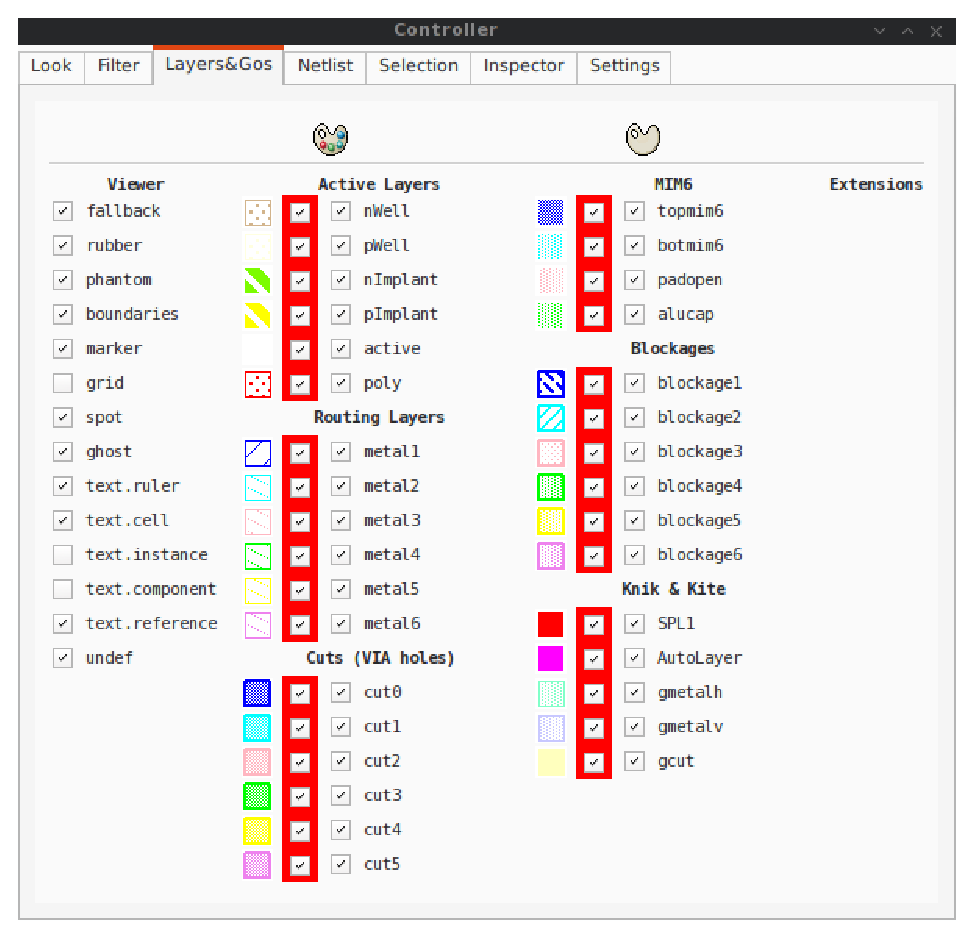
\includegraphics[width=.7\textwidth]{./images/Controller-1.eps}\end{center}}


%___________________________________________________________________________

\section*{Viewer \& Tools%
  \phantomsection%
  \addcontentsline{toc}{section}{Viewer \& Tools}%
  \label{id1}%
  \label{viewer-tools}%
}


%___________________________________________________________________________

\subsection*{The \DUrole{sc}{Hurricane} Data-Base%
  \phantomsection%
  \addcontentsline{toc}{subsection}{The Hurricane Data-Base}%
  \label{the-hurricane-data-base}%
}

The \DUrole{sc}{Alliance} flow is based on the \DUrole{sc}{mbk} data-base, which has one data-structure
for each view. That is, \DUrole{cb}{Lofig} for the \emph{logical} view and \DUrole{cb}{Phfig} for the \emph{physical}
view. The place and route tools were responsible for maintaining (or not) the
coherency between views. Reflecting this weak coupling between views, each one
was stored in a separate file with a specific format. The \emph{logical} view is stored
in a \DUrole{cb}{vst} file in \DUrole{sc}{vhdl} format and the \emph{physical} in an \DUrole{cb}{ap} file in an ad-hoc format.

The \DUrole{sc}{Coriolis} flow is based on the \DUrole{sc}{Hurricane} data-base, which has a unified
structure for \emph{logical} and \emph{physical} view. That data structure is the \emph{Cell} object.
The \emph{Cell} can have any state between pure netlist and completly placed and
routed design. Although the memory representation of the views has deeply
changed we still use the \DUrole{sc}{Alliance} files format, but they now really represent
views of the same object. The point is that one must be very careful about
view coherency when going to and from \DUrole{sc}{Coriolis}.

As for the first release, \DUrole{sc}{Coriolis} can be used only for two purposes :
%
\begin{itemize}

\item \textbf{Routing a design}, in that case the \emph{netlist}
view and the \emph{layout} view must be present and  \emph{layout} view must contain
a placement. Both views must have the same name. When saving the routed design,
it is advised to change the design name otherwise the original unrouted placement
in the \emph{layout} view will be overwritten.

\item \textbf{Viewing a design}, the \emph{netlist} view must be present, if a \emph{layout}
view is present it still must have the same name but it can be in any
state.

\end{itemize}


%___________________________________________________________________________

\subsection*{Mauka -{}- Placer%
  \phantomsection%
  \addcontentsline{toc}{subsection}{Mauka -{}- Placer}%
  \label{mauka-placer}%
}

Mauka makes uses of hMetis.

To be completed...

\DUadmonition[note]{
\DUtitle[note]{Note}

\emph{Instance Duplication Problem:} a same logical instance cannot have
two different placements. So, either you manually make a clone of it or you
supply a placement for it. This is currently a drawback of our \emph{folded hierarchy}
approach.
}


%___________________________________________________________________________

\subsection*{Knik -{}- Global Router%
  \phantomsection%
  \addcontentsline{toc}{subsection}{Knik -{}- Global Router}%
  \label{knik-global-router}%
}

The global router is (not yet) deterministic. To circumvent this limitation,
a global routing (also called a \emph{solution}) can be saved to disk and reloaded
for later uses.

A global routing is saved into a file with the same name as the design and a
\DUrole{cb}{kgr} extention. It is in \href{http://www.cerc.utexas.edu/~thyeros/boxrouter/boxrouter.htm}{Box Router} output format.

For an in-depth description of \DUrole{sc}{Knik} algorithms, you may download the thesis of
D. \DUrole{sc}{Dupuis} avalaible from here\textasciitilde{}: \href{http://www-soc.lip6.fr/en/users/damiendupuis/PhD/}{Knik Thesis}.
\DUrole{raw-latex}{\medskip}

\DUrole{raw-latex}{\noindent} Menus:
%
\begin{itemize}

\item \DUrole{raw-latex}{\fbox{\textsf{\textbf{{P\&R}}}}} \DUrole{raw-latex}{$\rightarrow$} \DUrole{raw-latex}{\fbox{\textsf{\textbf{{\underline{S}tep by Step}}}}} \DUrole{raw-latex}{$\rightarrow$} \DUrole{raw-latex}{\fbox{\textsf{\textbf{{\underline{S}ave Global Routing}}}}}.

\item \DUrole{raw-latex}{\fbox{\textsf{\textbf{{P\&R}}}}} \DUrole{raw-latex}{$\rightarrow$} \DUrole{raw-latex}{\fbox{\textsf{\textbf{{\underline{S}tep by Step}}}}} \DUrole{raw-latex}{$\rightarrow$} \DUrole{raw-latex}{\fbox{\textsf{\textbf{{\underline{L}oad Global Routing}}}}}.

\end{itemize}


%___________________________________________________________________________

\subsection*{Kite -{}- Detailed Router%
  \phantomsection%
  \addcontentsline{toc}{subsection}{Kite -{}- Detailed Router}%
  \label{kite-detailed-router}%
}

\DUrole{sc}{Kite} no longer suffers from the limitations of \DUrole{sc}{Nero}. It can route big designs
as its runtime and memory footprint is almost linear (with respect to the number
of gates). It has successfully routed design of more than \DUroletitlereference{150K} gates.
\DUrole{raw-latex}{\medskip}

\DUrole{raw-latex}{\noindent} However, this first release has the following restrictions:
%
\begin{itemize}

\item Works only with \DUrole{sc}{SxLib} standard cell gauge.

\item Works always with 4 routing metal layers (\DUroletitlereference{M2} through \DUroletitlereference{M5}).

\item Do not allow (take into account) pre-routed wires on signals
other than \DUrole{sc}{power} or \DUrole{sc}{ground}.

\end{itemize}

After each run, \DUrole{sc}{Kite} displays a set of \emph{completion ratios} which must all
be equal to \DUroletitlereference{100\%} if the detailed routing has been successfull.
In the event of a failure, on saturated design, you may decrease the
\DUroletitlereference{edge saturation ration} (argument \DUroletitlereference{-{}-edge}) to balance more evenly the design
saturation. That is, the maximum saturation decrease at the price of a wider
saturated area and increased wirelength.

\DUrole{raw-latex}{\newpage}

Routing a design is done in three ordered steps:
\setcounter{listcnt0}{0}
\begin{list}{\arabic{listcnt0}.}
{
\usecounter{listcnt0}
\setlength{\rightmargin}{\leftmargin}
}

\item Global routing   \DUrole{raw-latex}{\fbox{\textsf{\textbf{{P\&R}}}}} \DUrole{raw-latex}{$\rightarrow$} \DUrole{raw-latex}{\fbox{\textsf{\textbf{{\underline{S}tep by Step}}}}} \DUrole{raw-latex}{$\rightarrow$} \DUrole{raw-latex}{\fbox{\textsf{\textbf{{\underline{G}lobal Route}}}}}.

\item Detailed routing \DUrole{raw-latex}{\fbox{\textsf{\textbf{{P\&R}}}}} \DUrole{raw-latex}{$\rightarrow$} \DUrole{raw-latex}{\fbox{\textsf{\textbf{{\underline{S}tep by Step}}}}} \DUrole{raw-latex}{$\rightarrow$} \DUrole{raw-latex}{\fbox{\textsf{\textbf{{\underline{D}etailed Route}}}}}.

\item Finalize routing \DUrole{raw-latex}{\fbox{\textsf{\textbf{{P\&R}}}}} \DUrole{raw-latex}{$\rightarrow$} \DUrole{raw-latex}{\fbox{\textsf{\textbf{{\underline{S}tep by Step}}}}} \DUrole{raw-latex}{$\rightarrow$} \DUrole{raw-latex}{\fbox{\textsf{\textbf{{\underline{F}inalize Route}}}}}.
\end{list}

After the detailed routing step the \DUrole{sc}{Kite} data-structure is still active.
The wiring is thus represented in a way that allows \DUrole{sc}{Kite} to manage it but
which is not completly finished. The finalize step performs the removal of
the \DUrole{sc}{Kite} data-structure and finish/cleanup the wiring so that its
connex in the sense of \DUrole{sc}{Hurricane}. \emph{Do not} try to save
your design before that step, you would get gaps in it.

The complete description of \DUrole{sc}{Kite} parameters are described in \hyperref[detailed-routing-configuration-parameters]{Detailed Routing Configuration Parameters}.


%___________________________________________________________________________

\subsection*{Executing Python Scripts in Cgt%
  \phantomsection%
  \addcontentsline{toc}{subsection}{Executing Python Scripts in Cgt}%
  \label{executing-python-scripts-in-cgt}%
  \label{python-scripts-in-cgt}%
}

Python/Stratus scripts can be executed either in text or graphical mode.

\DUadmonition[note]{
\DUtitle[note]{Note}

\emph{How Cgt Locates Python Scripts.}
\DUrole{cb}{cgt} uses the Python \texttt{import} mechanism to load Python scripts.
So you must give the name of your script whitout \texttt{.py} extention and
it must be reachable through the \texttt{PYTHONPATH}. You may uses the
dotted module notation.
}

A Python/Stratus script must contains a function called \texttt{StratusScript}
with one optional argument, the graphical editor into which it may be
running (will be set to \texttt{None} in text mode).

Any script given on the command line will be run immediatly \emph{after} the
initializations and \emph{before} any other argument is processed.

Small example of Python/Stratus script:
%
\begin{quote}{\ttfamily \raggedright \noindent
from~status~import~*\\
~\\
def~doSomething~():\\
~~~~\#~...\\
~~~~return\\
~\\
def~StratusScript~(~editor=None~):\\
~~if~globals().has\_key~(~"\_\_editor"~):~editor~=~\_\_editor\\
~~if~editor:~setEditor~(~editor~)\\
~\\
~~doSomething()\\
~~return\\
~\\
if~\_\_name\_\_~==~"\_\_main\_\_"~:\\
~~StratusScript~()
}
\end{quote}

This script could be run directly with Python (thanks to the two last lines)
or through \DUrole{cb}{cgt} in both text and graphical modes.


%___________________________________________________________________________

\subsection*{Printing \& Snapshots%
  \phantomsection%
  \addcontentsline{toc}{subsection}{Printing \& Snapshots}%
  \label{printing-snapshots}%
}

Printing or saving into a \DUrole{sc}{pdf} is fairly simple, just uses the \textbf{File -> Print}
menu or the \DUrole{raw-latex}{\key{CTRL}\xspace} \DUrole{raw-latex}{$+$\xspace} \DUrole{raw-latex}{\key{p}\xspace} shortcut to open the dialog box.

The print functionality uses exactly the same rendering mechanism as for the
screen, beeing almost \emph{WYSIWYG}. Thus, to obtain the best results it is advisable
to select the \texttt{Coriolis.Printer} look (in the \emph{Controller}), which uses a
white background and much suited for high resolutions \texttt{32x32} pixels patterns

There is also two mode of printing selectable through the \emph{Controller}
\textbf{Settings -> Misc -> Printer/Snapshot Mode}:

\leavevmode
\setlength{\DUtablewidth}{\linewidth}
\begin{longtable}[c]{|p{0.174\DUtablewidth}|p{0.195\DUtablewidth}|p{0.576\DUtablewidth}|}
\hline

Mode
 & 
DPI (approx.)
 & 
Intended Usage
 \\
\hline

\textbf{Cell Mode}
 & 
150
 & 
For single \texttt{Cell} printing or very small designs.
Patterns will be bigger and more readable.
 \\
\hline

\textbf{Design Mode}
 & 
300
 & 
For designs (mostly commposed of wires and cells
outlines).
 \\
\hline
\end{longtable}

\DUadmonition[note]{
\DUtitle[note]{Note}

\emph{The pdf file size}
Be aware that the generated \DUrole{sc}{pdf} files are indeed only pixmaps.
So they can grew very large if you select paper format above \texttt{A2}
or similar.
}

\DUrole{raw-latex}{\noindent}
Saving into an image is subject to the same remarks as for \DUrole{sc}{pdf}.


%___________________________________________________________________________

\subsection*{Memento of Shortcuts in Graphic Mode%
  \phantomsection%
  \addcontentsline{toc}{subsection}{Memento of Shortcuts in Graphic Mode}%
  \label{memento-of-shortcuts-in-graphic-mode}%
}

The main application binary is \DUrole{cb}{cgt}.

\leavevmode
\setlength{\DUtablewidth}{\linewidth}
\begin{longtable}[c]{|p{0.160\DUtablewidth}|p{0.199\DUtablewidth}|p{0.586\DUtablewidth}|}
\hline
\textbf{%
Category
} & \textbf{%
Keys
} & \textbf{%
Action
} \\
\hline
\endfirsthead
\hline
\textbf{%
Category
} & \textbf{%
Keys
} & \textbf{%
Action
} \\
\hline
\endhead
\multicolumn{3}{c}{\hfill ... continued on next page} \\
\endfoot
\endlastfoot

\textbf{Moves}
 & 
\begin{DUlineblock}{0em}
\item[] \DUrole{raw-latex}{\key{Up}\xspace},
\DUrole{raw-latex}{\key{Down}\xspace}
\item[] \DUrole{raw-latex}{\key{Left}\xspace},
\DUrole{raw-latex}{\key{Right}\xspace}
\end{DUlineblock}
 & 
Shift the view in the according direction
 \\
\hline

\textbf{Fit}
 & 
\DUrole{raw-latex}{\key{f}\xspace}
 & 
Fit to the Cell abutment box
 \\
\hline

\textbf{Refresh}
 & 
\DUrole{raw-latex}{\key{CTRL}\xspace}
\DUrole{raw-latex}{$+$\xspace} \DUrole{raw-latex}{\key{l}\xspace}
 & 
Triggers a complete display redraw
 \\
\hline

\textbf{Goto}
 & 
\DUrole{raw-latex}{\key{G}\xspace}
 & 
\emph{apperture} is the minimum side of the area
displayed around the point to go to. It's an
alternative way of setting the zoom level
 \\
\hline
\multirow{2}{0.16\DUtablewidth}{%
\textbf{Zoom}
} & 
\DUrole{raw-latex}{\key{z}\xspace},
\DUrole{raw-latex}{\key{m}\xspace}
 & 
Respectively zoom by a 2 factor and \emph{unzoom}
by a 2 factor
 \\
\cline{2-2}
\cline{3-3}
 & 
\begin{DUlineblock}{0em}
\item[] 
\includegraphics[scale=0.250000]{./images/ComputerMouse.png}
\item[] Area Zoom
\end{DUlineblock}
 & 
You can perform a zoom to an area.
Define the zoom area by \emph{holding down the left
mouse button} while moving the mouse.
 \\
\hline
\multirow{3}{0.16\DUtablewidth}{%
\textbf{Selection}
} & 
\begin{DUlineblock}{0em}
\item[] 
\includegraphics[scale=0.250000]{./images/ComputerMouse.png}
\item[] Area Selection
\end{DUlineblock}
 & 
You can select displayed objects under an area.
Define the selection area by \emph{holding down the
right mouse button} while moving the mouse.
 \\
\cline{2-2}
\cline{3-3}
 & 
\begin{DUlineblock}{0em}
\item[] 
\includegraphics[scale=0.250000]{./images/ComputerMouse.png}
\item[] Toggle Selection
\end{DUlineblock}
 & 
You can toggle the selection of one object under
the mouse position by pressing \DUrole{raw-latex}{\key{CTRL}\xspace} and
pressing down \emph{the right mouse button}. A popup
list of what's under the position shows up into
which you can toggle the selection state of one
item.
 \\
\cline{2-2}
\cline{3-3}
 & 
\DUrole{raw-latex}{\key{S}\xspace}
 & 
Toggle  the selection visibility
 \\
\hline

\textbf{Controller}
 & 
\DUrole{raw-latex}{\key{CTRL}\xspace}
\DUrole{raw-latex}{$+$\xspace} \DUrole{raw-latex}{\key{i}\xspace}
 & 
Show/hide the controller window.

It's the Swiss Army Knife of the viewer.
From it, you can fine-control the display and
inspect almost everything in your design.
 \\
\hline
\multirow{2}{0.16\DUtablewidth}{%
\textbf{Rulers}
} & 
\DUrole{raw-latex}{\key{k}\xspace},
\DUrole{raw-latex}{\key{ESC}\xspace}
 & 
One stroke on \DUrole{raw-latex}{\key{k}\xspace} enters the ruler mode, in
which you can draw one ruler. You can exit the
ruler mode by pressing \DUrole{raw-latex}{\key{ESC}\xspace}. Once in ruler
mode, the first click on the \emph{left mouse button}
sets the ruler's starting point and the second
click the ruler's end point. The second click
exits automatically the ruler mode.
 \\
\cline{2-2}
\cline{3-3}
 & 
\DUrole{raw-latex}{\key{K}\xspace}
 & 
Clears all the drawn rulers
 \\
\hline

\textbf{Print}
 & 
\DUrole{raw-latex}{\key{CTRL}\xspace}
\DUrole{raw-latex}{$+$\xspace} \DUrole{raw-latex}{\key{p}\xspace}
 & 
Currently rather crude. It's a direct copy of
what's displayed in pixels. So the resulting
picture will be a little blurred due to
anti-aliasing mechanism.
 \\
\hline
\multirow{3}{0.16\DUtablewidth}{%
\textbf{Open/Close}
} & 
\DUrole{raw-latex}{\key{CTRL}\xspace}
\DUrole{raw-latex}{$+$\xspace} \DUrole{raw-latex}{\key{o}\xspace}
 & 
Opens a new design. The design name must be
given without path or extention.
 \\
\cline{2-2}
\cline{3-3}
 & 
\DUrole{raw-latex}{\key{CTRL}\xspace}
\DUrole{raw-latex}{$+$\xspace} \DUrole{raw-latex}{\key{w}\xspace}
 & 
Close the current viewer window, but do not quit
the application.
 \\
\cline{2-2}
\cline{3-3}
 & 
\DUrole{raw-latex}{\key{CTRL}\xspace}
\DUrole{raw-latex}{$+$\xspace} \DUrole{raw-latex}{\key{q}\xspace}
 & 
\DUroletitlereference{CTRL+Q} quit the application
(closing all windows).
 \\
\hline
\multirow{2}{0.16\DUtablewidth}{%
\textbf{Hierarchy}
} & 
\DUrole{raw-latex}{\key{CTRL}\xspace} \DUrole{raw-latex}{$+$\xspace}
\DUrole{raw-latex}{\key{Down}\xspace}
 & 
Go one hierarchy level down. That is, if there
is an \emph{instance} under the cursor position, load
it's \emph{model} Cell in place of the current one.
 \\
\cline{2-2}
\cline{3-3}
 & 
\DUrole{raw-latex}{\key{CTRL}\xspace} \DUrole{raw-latex}{$+$\xspace}
\DUrole{raw-latex}{\key{Up}\xspace}
 & 
Go one hierarchy level up. if we have entered
the current model through \DUrole{raw-latex}{\key{CTRL}\xspace} \DUrole{raw-latex}{$+$\xspace}
\DUrole{raw-latex}{\key{Down}\xspace}, reload the previous model (the one
in which this model is instanciated).
 \\
\hline
\end{longtable}


%___________________________________________________________________________

\subsection*{Cgt Command Line Options%
  \phantomsection%
  \addcontentsline{toc}{subsection}{Cgt Command Line Options}%
  \label{cgt-command-line-options}%
}

Appart from the obvious \texttt{-{}-text} options, all can be used for text and graphical mode.

\leavevmode
\setlength{\DUtablewidth}{\linewidth}
\begin{longtable}[c]{|p{0.354\DUtablewidth}|p{0.575\DUtablewidth}|}
\hline
\textbf{%
Arguments
} & \textbf{%
Meaning
} \\
\hline
\endfirsthead
\hline
\textbf{%
Arguments
} & \textbf{%
Meaning
} \\
\hline
\endhead
\multicolumn{2}{c}{\hfill ... continued on next page} \\
\endfoot
\endlastfoot

\DUroletitlereference{-t|-{}-text}
 & 
Instruct \DUrole{cb}{cgt} to run in text mode.
 \\
\hline

\DUroletitlereference{-L|-{}-log-mode}
 & 
Disable the uses of \DUrole{sc}{ansi} escape sequence on
the \DUrole{cb}{tty}. Useful when the output is
redirected to a file.
 \\
\hline

\DUroletitlereference{-c <cell>|-{}-cell=<cell>}
 & 
The name of the design to load, without
leading path or extention.
 \\
\hline

\DUroletitlereference{-g|-{}-load-global}
 & 
Reload a global routing solution from disk.
The file containing the solution must be named
\DUroletitlereference{<cell>.kgr}.
 \\
\hline

\DUroletitlereference{-{}-save-global}
 & 
Save the global routing solution, into a file
named \DUroletitlereference{<design>.kgr}.
 \\
\hline

\DUroletitlereference{-e <ratio>|-{}-edge=<ratio>}
 & 
Change the edge capacity for the global
router, between 0 and 1 (\DUrole{sc}{Knik}).
 \\
\hline

\DUroletitlereference{-G|-{}-global-route}
 & 
Run the global router (\DUrole{sc}{Knik}).
 \\
\hline

\DUroletitlereference{-R|-{}-detailed-route}
 & 
Run the detailed router (\DUrole{sc}{Kite}).
 \\
\hline

\DUroletitlereference{-s|-{}-save-design=<routed>}
 & 
The design into which the routed layout will
be saved. It is strongly recommanded to choose
a different name from the source (unrouted)
design.
 \\
\hline

\DUroletitlereference{-{}-events-limit=<count>}
 & 
The maximal number of events after which the
router will stops. This is mainly a failsafe
against looping. The limit is sets to 4
millions of iteration which should suffice to
any design of \DUroletitlereference{100K}. gates. For bigger
designs you may wants to increase this limit.
 \\
\hline

\DUroletitlereference{-{}-stratus-script=<module>}
 & 
Run the Python/Stratus script \texttt{module}.
See \hyperref[python-scripts-in-cgt]{Python Scripts in Cgt}.
 \\
\hline
\end{longtable}

Some Examples :
%
\begin{itemize}

\item Run both global and detailed router, then save the routed design :
%
\begin{quote}{\ttfamily \raggedright \noindent
>~cgt~-v~-t~-G~-R~-{}-cell=design~-{}-save-design=design\_kite
}
\end{quote}

\item Load a previous global solution, run the detailed router, then save the
routed design :
%
\begin{quote}{\ttfamily \raggedright \noindent
>~cgt~-v~-t~-{}-load-global~-R~-{}-cell=design~-{}-save-design=design\_kite
}
\end{quote}

\item Run the global router, then save the global routing solution :
%
\begin{quote}{\ttfamily \raggedright \noindent
>~cgt~-v~-t~-G~-{}-save-global~-{}-cell=design
}
\end{quote}

\end{itemize}


%___________________________________________________________________________

\section*{The Controller%
  \phantomsection%
  \addcontentsline{toc}{section}{The Controller}%
  \label{id2}%
  \label{the-controller}%
}

The \emph{Controller} window is composed of seven tabs:
\setcounter{listcnt0}{0}
\begin{list}{\arabic{listcnt0}.}
{
\usecounter{listcnt0}
\setlength{\rightmargin}{\leftmargin}
}

\item \hyperref[the-look-tab]{The Look Tab} to select the display style.

\item \hyperref[the-filter-tab]{The Filter Tab} the hierarchical levels to be displayed, the look of
rubbers and the dimension units.

\item \hyperref[the-layers-go-tab]{The Layers\&Go Tab} to selectively hide/display layers.

\item \hyperref[the-netlist-tab]{The Netlist Tab} to browse through the \emph{netlist}. Works in association
with the \emph{Selection} tab.

\item \hyperref[the-selection-tab]{The Selection Tab} allow to view all the currently selected elements.

\item \hyperref[the-inspector-tab]{The Inspector Tab} browse through either the DataBase, the Cell or
the current selection.

\item \hyperref[the-settings-tab]{The Settings Tab} access all the tool's configuration settings.
\end{list}


%___________________________________________________________________________

\subsection*{The Look Tab%
  \phantomsection%
  \addcontentsline{toc}{subsection}{The Look Tab}%
  \label{id3}%
  \label{the-look-tab}%
}

You can select how the layout will be displayed. There is a special one
\texttt{Printer.Coriolis} specifically designed for \hyperref[printing-snapshots]{Printing \& Snapshots}.
You should select it prior to calling the print or snapshot dialog boxes.

\DUrole{raw-latex}{\begin{center}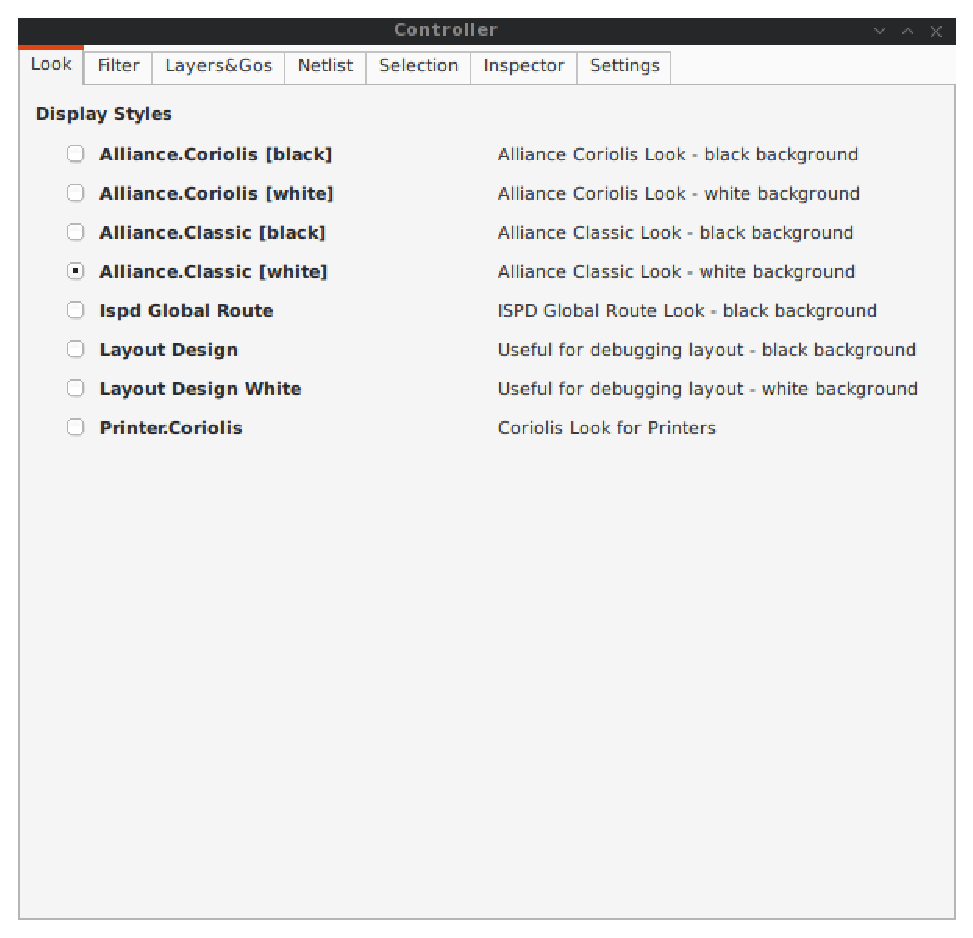
\includegraphics[width=.7\textwidth]{./images/Controller-Look-1.eps}\end{center}}


%___________________________________________________________________________

\subsection*{The Filter Tab%
  \phantomsection%
  \addcontentsline{toc}{subsection}{The Filter Tab}%
  \label{id4}%
  \label{the-filter-tab}%
}

The filter tab let you select what hierarchical levels of your design will be
displayed. Hierarchy level are numbered top-down: the level 0 correspond to
the top-level cell, the level one to the instances of the top-level Cell and
so on.

There are also check boxes to enable/disable the processing of Terminal Cell,
Master Cells and Compnents. The processing of Terminal Cell (hierarchy leaf
cells) is disabled by default when you load a hierarchical design and enabled
when you load a single Cell.

You can choose what kind of form to give to the rubbers and the type of
unit used to display coordinates.

\DUadmonition[note]{
\DUtitle[note]{Note}

\emph{What are Rubbers:} \DUrole{sc}{Hurricane} uses \emph{Rubbers} to materialize
physical gaps in net topology. That is, if some wires are missing to
connect two or more parts of net, a \emph{rubber} will be drawn between them
to signal the gap.

For example, after the detailed routing no \emph{rubbers} should remains.
They have been made \emph{very} visibles as big violet lines...
}

\DUrole{raw-latex}{\begin{center}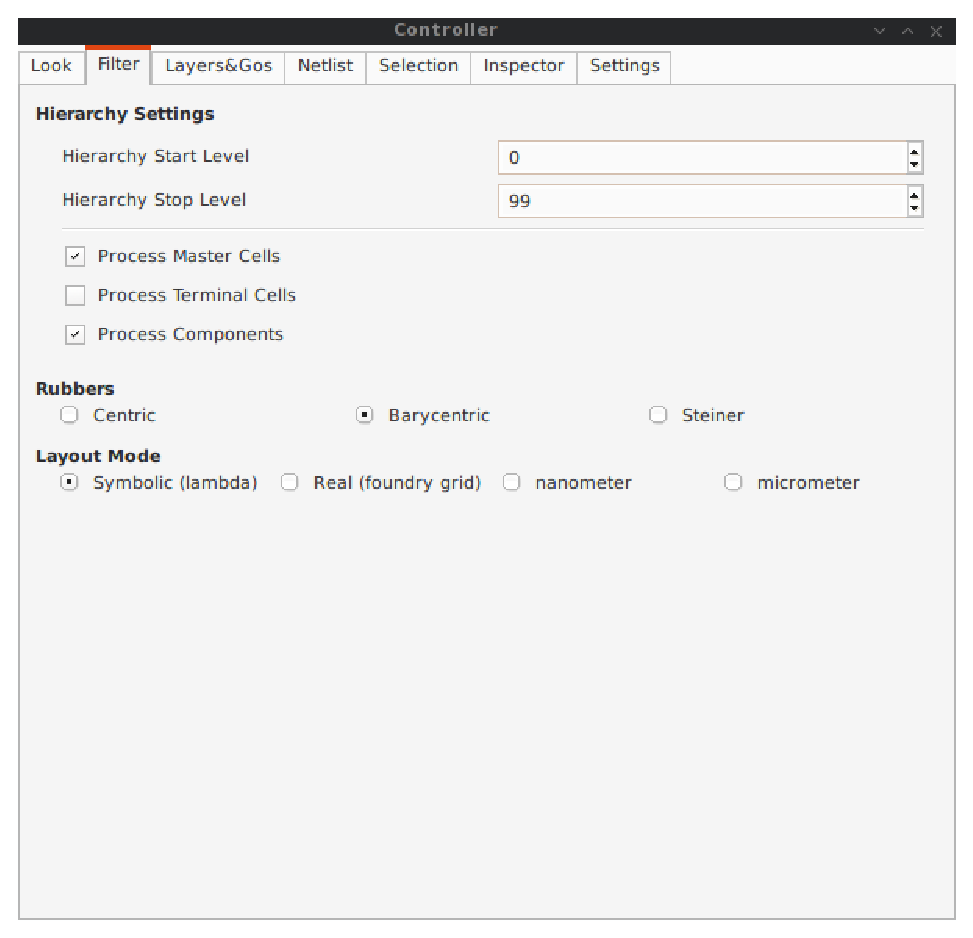
\includegraphics[width=.7\textwidth]{./images/Controller-Filter-1.eps}\end{center}}


%___________________________________________________________________________

\subsection*{The Layers\&Go Tab%
  \phantomsection%
  \addcontentsline{toc}{subsection}{The Layers\&Go Tab}%
  \label{id5}%
  \label{the-layers-go-tab}%
}

Control the individual display of all \emph{layers} and \emph{Gos}.
%
\begin{itemize}

\item \emph{Layers} correspond to a true physical layer. From a \DUrole{sc}{Hurricane} point of
view they are all the \emph{BasicLayers} (could be matched to GDSII).

\item \emph{Gos} stands from \emph{Graphical Objects}, they are drawings that have no
physical existence but are added by the various tools to display extra
information. One good exemple is the density map of the detailed router,
to easily locate congested areas.

\end{itemize}

For each layer/Go there are two check boxes:
%
\begin{itemize}

\item The normal one triggers the display.

\item The red-outlined allows objects of that layer to be selectable or not.

\end{itemize}

\DUrole{raw-latex}{\begin{center}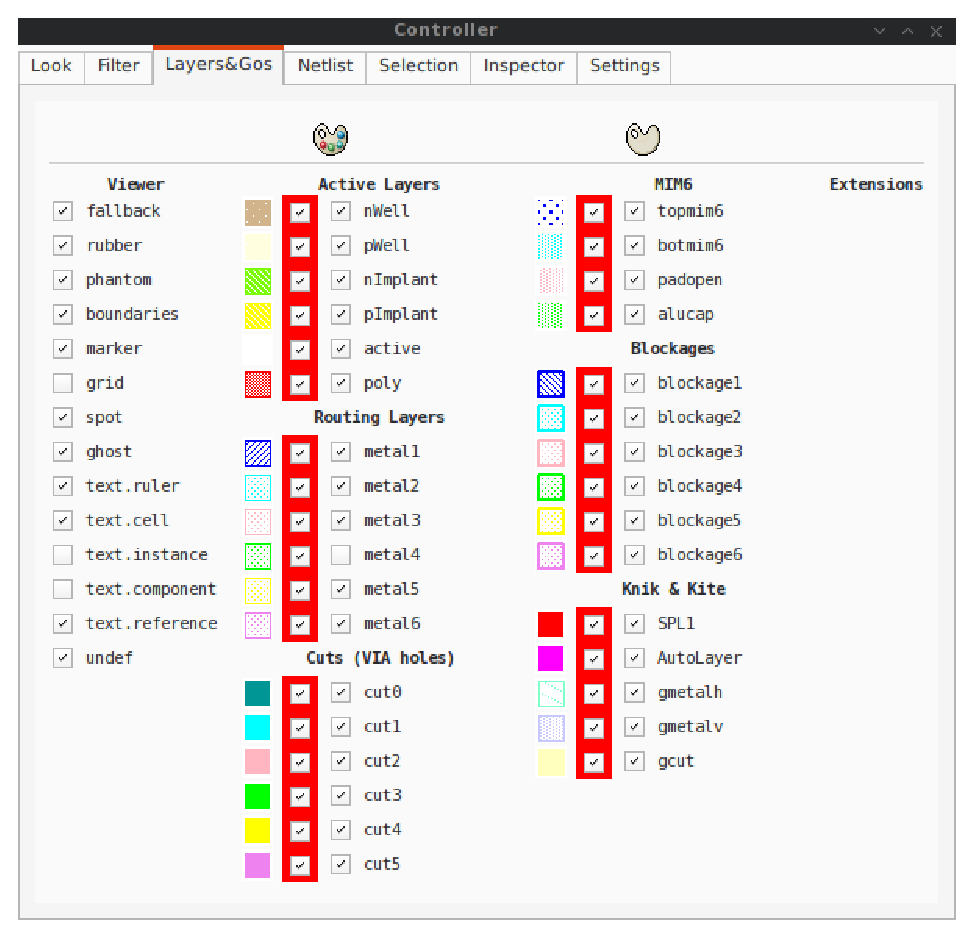
\includegraphics[width=.7\textwidth]{./images/Controller-LayersGos-1.eps}\end{center}}


%___________________________________________________________________________

\subsection*{The Netlist Tab%
  \phantomsection%
  \addcontentsline{toc}{subsection}{The Netlist Tab}%
  \label{id6}%
  \label{the-netlist-tab}%
}

The \emph{Netlist} tab shows the list of nets... By default the tab is not
\emph{synched} with the displayed Cell. To see the nets you must check the
\textbf{Sync Netlist} checkbox. You can narrow the set of displayed nets by
using the filter pattern (supports regular expressions).

An very useful feature is to enable the \textbf{Sync Selection}, which will
automatically select all the components of the selected net(s). You can
select multiple nets. In the figure the net \texttt{auxsc35} is selected and
is highlited in the \emph{Viewer}.

\DUrole{raw-latex}{\begin{center}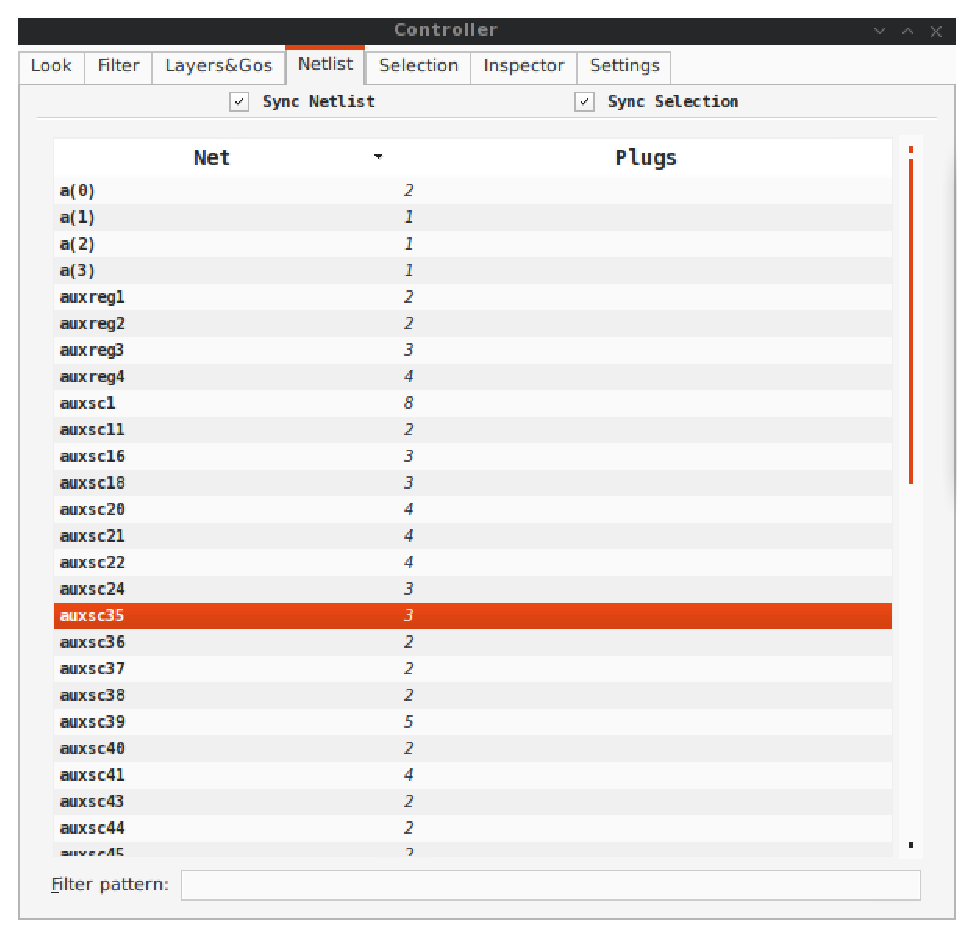
\includegraphics[width=.7\textwidth]{./images/Controller-Netlist-1.eps}\end{center}}
\DUrole{raw-latex}{\begin{center}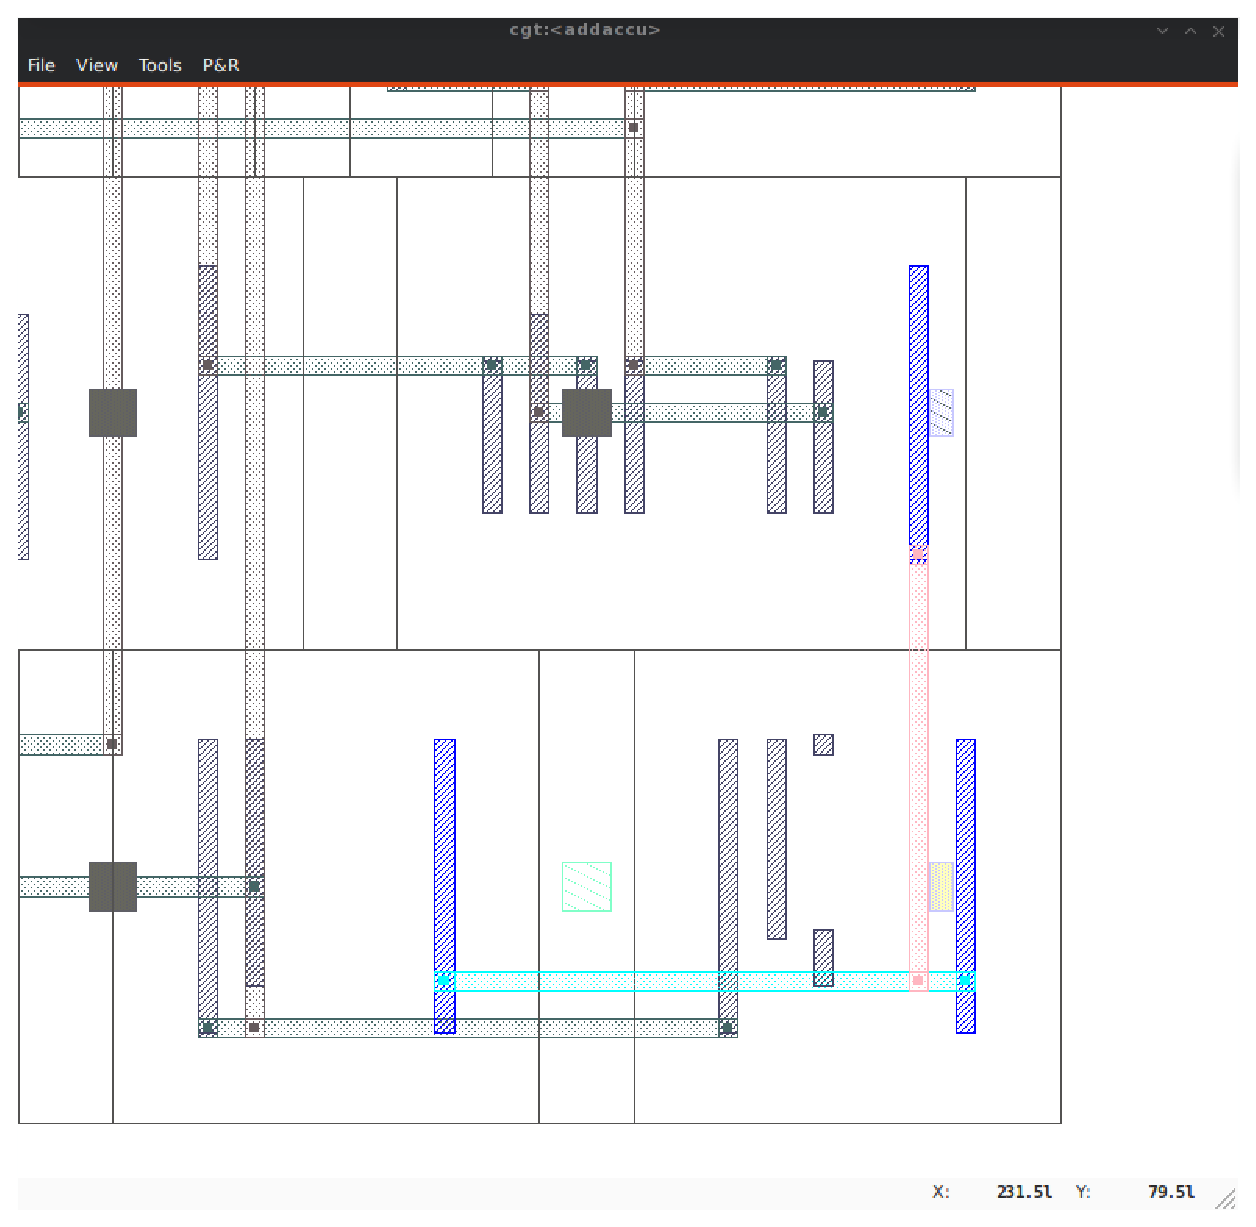
\includegraphics[width=.7\textwidth]{./images/Viewer-Netlist-1.eps}\end{center}}


%___________________________________________________________________________

\subsection*{The Selection Tab%
  \phantomsection%
  \addcontentsline{toc}{subsection}{The Selection Tab}%
  \label{id7}%
  \label{the-selection-tab}%
}

The \emph{Selection} tab list all the components currently selecteds. They
can be filtered thanks to the filter pattern.

Used in conjunction with the \emph{Netlist} \textbf{Sync Selection} you will all see
all the components part of \emph{net}.

In this list, you can toggle individually the selection of component by
pressing the \texttt{t} key. When unselected in this way a component is not
removed from the the selection list but instead displayed in red italic.
To see where a component is you may make it blink by repeatedly press
the \texttt{t} key...

\DUrole{raw-latex}{\begin{center}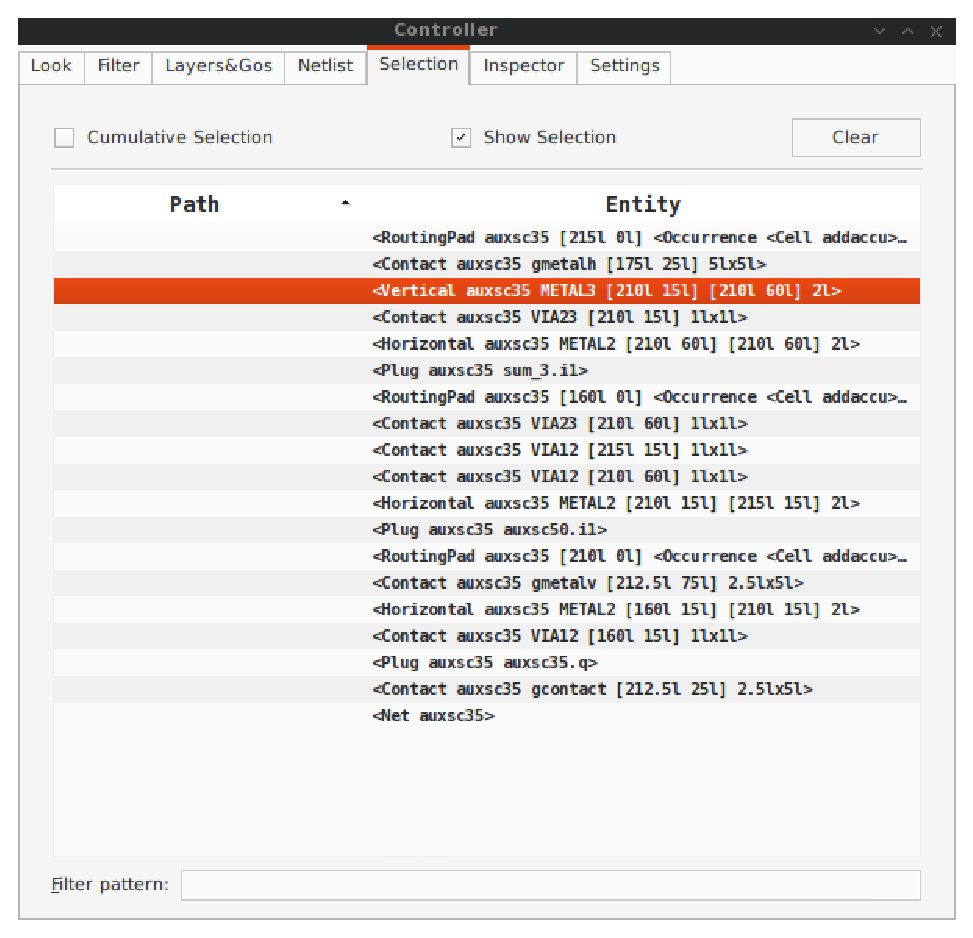
\includegraphics[width=.7\textwidth]{./images/Controller-Selection-1.eps}\end{center}}


%___________________________________________________________________________

\subsection*{The Inspector Tab%
  \phantomsection%
  \addcontentsline{toc}{subsection}{The Inspector Tab}%
  \label{id8}%
  \label{the-inspector-tab}%
}

This tab is very useful, but mostly for \DUrole{sc}{Coriolis} developpers. It allows
to browse through the live DataBase. The \emph{Inspector} provide three entry points:
%
\begin{itemize}

\item \textbf{DataBase}: Starts from the whole \DUrole{sc}{Hurricane} DataBase.

\item \textbf{Cell}: Inspect the currently loaded Cell.

\item \textbf{Selection}: Inspect the object currently highlited in the \emph{Selection} tab.

\end{itemize}

Once an entry point has been activated, you may recursively expore all
it's fields using the right/left arrows.

\DUadmonition[note]{
\DUtitle[note]{Note}

\emph{Do not put your fingers in the socket:} when inspecting
anything, do not modify the DataBase. If the any object under inspection
is deleted, you will crash the application...
}

\DUadmonition[note]{
\DUtitle[note]{Note}

\emph{Implementation Detail:} the inspector support is done with
\texttt{Slot}, \texttt{Record} and \texttt{getString()}.
}

\DUrole{raw-latex}{\begin{center}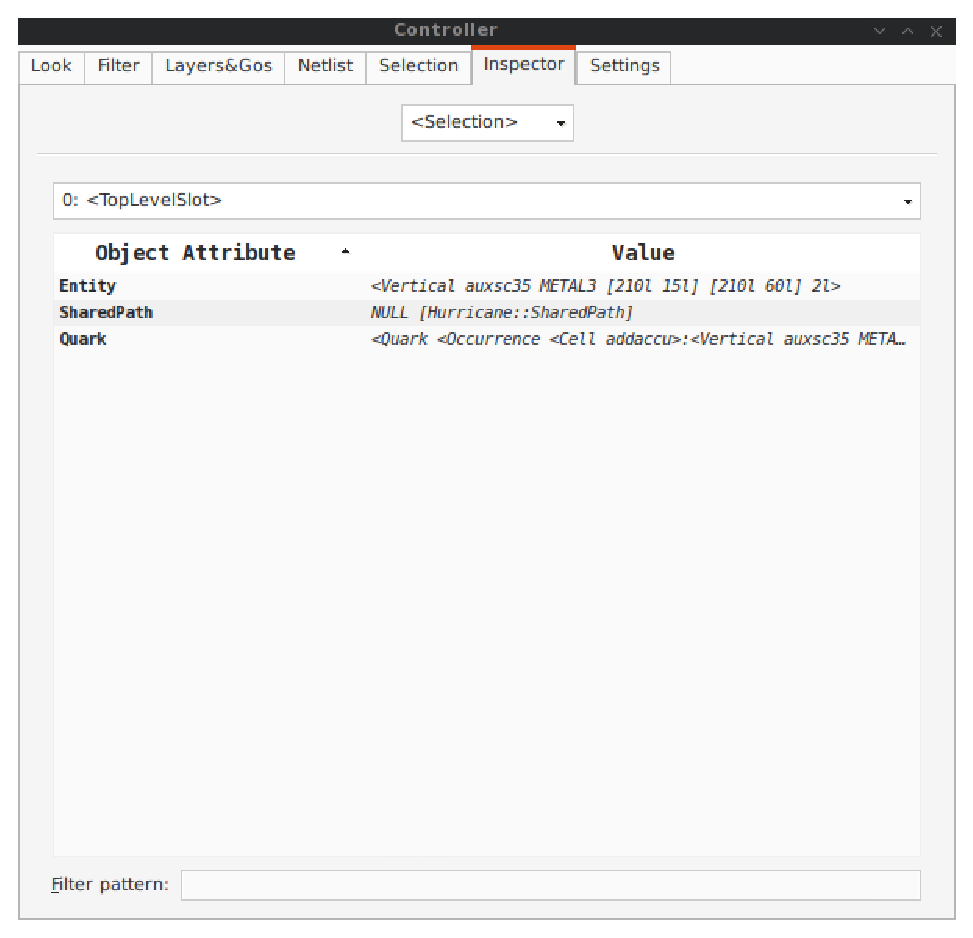
\includegraphics[width=.7\textwidth]{./images/Controller-Inspector-1.eps}\end{center}}
\DUrole{raw-latex}{\begin{center}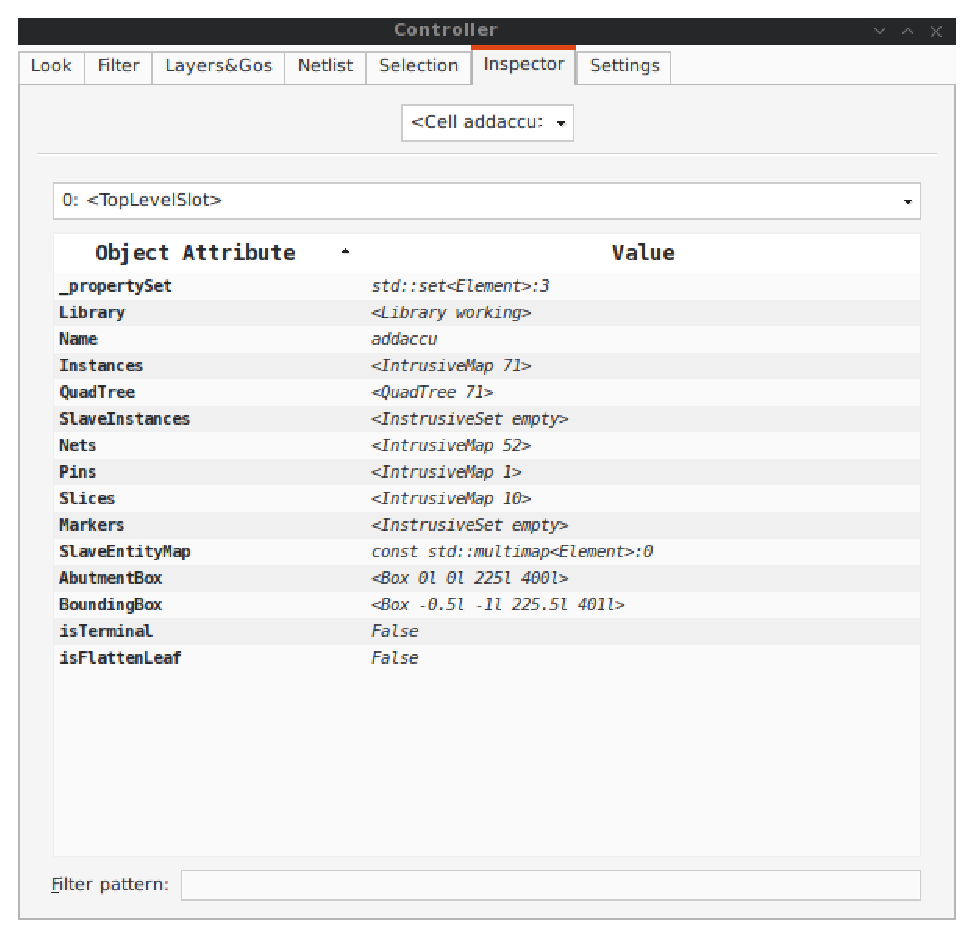
\includegraphics[width=.7\textwidth]{./images/Controller-Inspector-2.eps}\end{center}}
\DUrole{raw-latex}{\begin{center}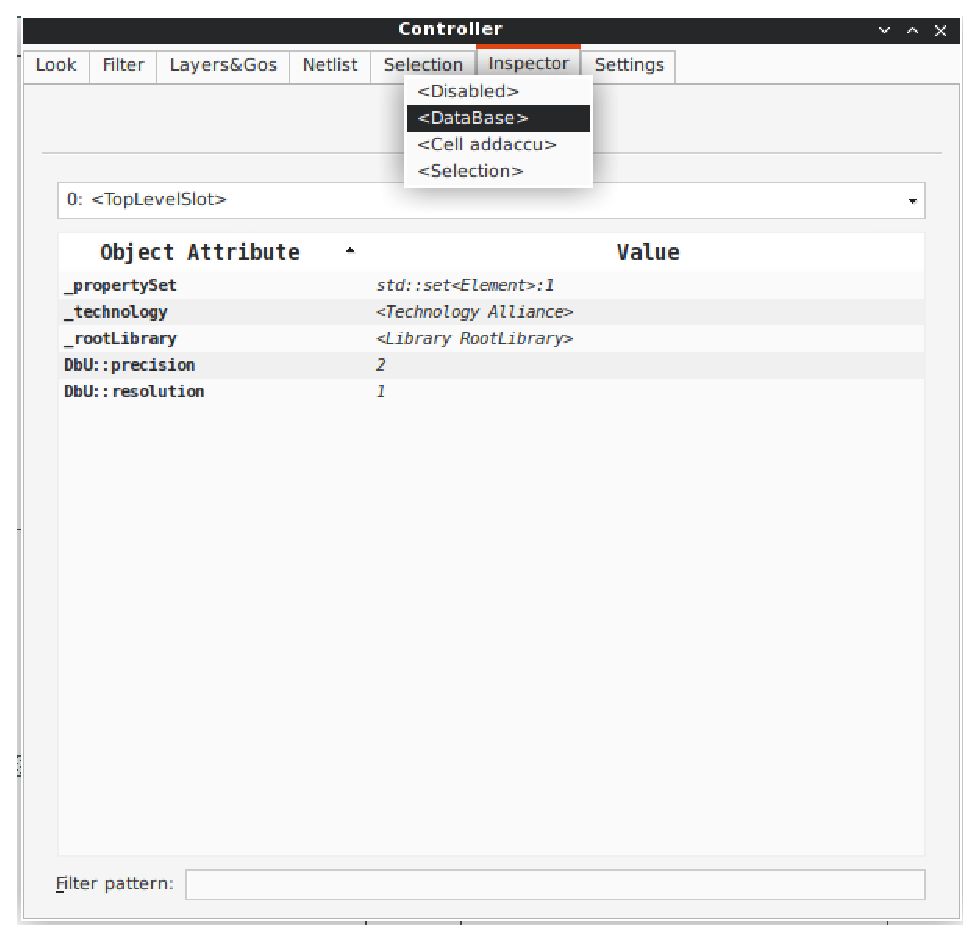
\includegraphics[width=.7\textwidth]{./images/Controller-Inspector-3.eps}\end{center}}


%___________________________________________________________________________

\subsection*{The Settings Tab%
  \phantomsection%
  \addcontentsline{toc}{subsection}{The Settings Tab}%
  \label{id9}%
  \label{the-settings-tab}%
}

Here comes the description of the \emph{Settings} tab.

\DUrole{raw-latex}{\begin{center}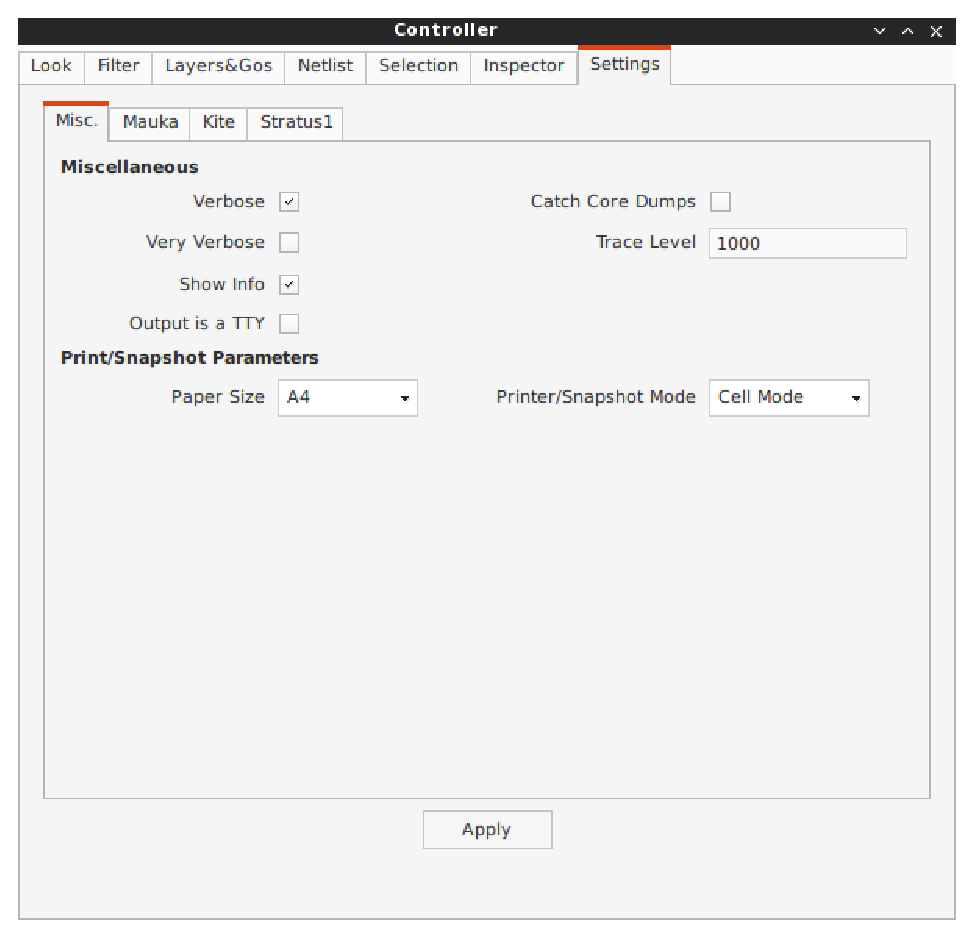
\includegraphics[width=.7\textwidth]{./images/Controller-Settings-1.eps}\end{center}}


%___________________________________________________________________________

\section*{Tools Fine Tuning%
  \phantomsection%
  \addcontentsline{toc}{section}{Tools Fine Tuning}%
  \label{tools-fine-tuning}%
}


%___________________________________________________________________________

\subsection*{Detailed Routing Configuration Parameters%
  \phantomsection%
  \addcontentsline{toc}{subsection}{Detailed Routing Configuration Parameters}%
  \label{id10}%
  \label{detailed-routing-configuration-parameters}%
}

\leavevmode
\setlength{\DUtablewidth}{\linewidth}
\begin{longtable}[c]{|p{0.470\DUtablewidth}|p{0.226\DUtablewidth}|p{0.145\DUtablewidth}|}
\hline
\textbf{%
Parameter Identifier
} & \textbf{%
Type
} & \textbf{%
Default
} \\
\hline
\endfirsthead
\hline
\textbf{%
Parameter Identifier
} & \textbf{%
Type
} & \textbf{%
Default
} \\
\hline
\endhead
\multicolumn{3}{c}{\hfill ... continued on next page} \\
\endfoot
\endlastfoot
\multicolumn{3}{|l|}{
\textbf{Katabatic Parameters}
} \\
\hline

\begin{DUlineblock}{0em}
\item[] \texttt{katabatic.globalLengthThreshold}
\item[] \texttt{katabatic.saturateRatio}
\item[] \texttt{katabatic.saturateRp}
\item[] \texttt{kite.borderRipupLimit}
\end{DUlineblock}
 & 
\begin{DUlineblock}{0em}
\item[] TypeInt
\item[] TypePercentage
\item[] TypeInt
\item[] TypeInt
\end{DUlineblock}
 & 
\begin{DUlineblock}{0em}
\item[] 1450
\item[] 80
\item[] 8
\item[] 26
\end{DUlineblock}
 \\
\hline
\multicolumn{3}{|l|}{
\textbf{Kite Parameters}
} \\
\hline

\begin{DUlineblock}{0em}
\item[] \texttt{kite.edgeCapacity}
\item[] \texttt{kite.eventsLimit}
\item[] \texttt{kite.ripupCost}
\item[] \texttt{kite.globalRipupLimit}
\item[] \texttt{kite.localRipupLimit}
\item[] \texttt{kite.longGlobalRipupLimit}
\item[] \texttt{kite.strapRipupLimit}
\item[] \texttt{kite.metal1MinBreak}
\item[] \texttt{kite.metal2MinBreak}
\item[] \texttt{kite.metal3MinBreak}
\item[] \texttt{kite.metal4MinBreak}
\item[] \texttt{kite.metal5MinBreak}
\item[] \texttt{kite.metal6MinBreak}
\item[] \texttt{kite.metal7MinBreak}
\end{DUlineblock}
 & 
\begin{DUlineblock}{0em}
\item[] TypePercentage
\item[] TypeInt
\item[] TypeInt
\item[] TypeInt
\item[] TypeInt
\item[] TypeInt
\item[] TypeInt
\item[] TypeDouble
\item[] TypeDouble
\item[] TypeDouble
\item[] TypeDouble
\item[] TypeDouble
\item[] TypeDouble
\item[] TypeDouble
\end{DUlineblock}
 & 
\begin{DUlineblock}{0em}
\item[] 65
\item[] 4000002
\item[] 3
\item[] 5
\item[] 7
\item[] 5
\item[] 16
\item[] 100
\item[] 100
\item[] 100
\item[] 1450
\item[] 1450
\item[] 1450
\item[] 1450
\end{DUlineblock}
 \\
\hline
\end{longtable}


%___________________________________________________________________________

\section*{Installation from Sources%
  \phantomsection%
  \addcontentsline{toc}{section}{Installation from Sources}%
  \label{id11}%
  \label{installation-from-sources}%
}

Installation from source is done differently than what is done in the packaging
procedure. The archive is also structured differently and meant to be unpacked
and compiled under a user's home directory.

Main building prerequisites:
%
\begin{itemize}

\item cmake

\item g++

\item boost

\item libxml2

\item yacc \& lex.

\item Qt 4

\item LEF/DEF (optional).

\item hMetis (optional).

\item doxygen.

\item latex

\item latex2html.

\item python-docutils (for reStructuredText).

\end{itemize}

Simple building procedure:
%
\begin{quote}{\ttfamily \raggedright \noindent
dummy@lepka:\textasciitilde{}\$~tar~jxvf~coriolis2-1.0-20121103.tar.bz2\\
dummy@lepka:\textasciitilde{}\$~cd~coriolis-2.x/src\\
dummy@lepka:src\$~./bootstrap/buildCoriolis.py~\textbackslash{}\\
~~~~~~~~~~~~~~~~~-{}-project=bootstrap~-{}-project=vlsisapd~-{}-project=coriolis~\textbackslash{}\\
~~~~~~~~~~~~~~~~~-{}-make="-j4~install"\\
dummy@lepka:src\$~./bootstrap/buildCoriolis.py~\textbackslash{}\\
~~~~~~~~~~~~~~~~~-{}-project=bootstrap~-{}-project=vlsisapd~-{}-project=coriolis~\textbackslash{}\\
~~~~~~~~~~~~~~~~~-{}-doc~-{}-make="-j1~install"
}
\end{quote}

Installation is done according to the following tree structure:

\leavevmode
\setlength{\DUtablewidth}{\linewidth}
\begin{longtable}[c]{|p{0.247\DUtablewidth}|p{0.693\DUtablewidth}|}
\hline

Linux, SL 6, 32 bits
 & 
\textasciitilde{}/coriolis-2.x/Linux.slsoc6x/Release.Shared/install
 \\
\hline

Linux, SL 6, 64 bits
 & 
\textasciitilde{}/coriolis-2.x/Linux.slsoc6x\_64/Release.Shared/install
 \\
\hline

FreeBSD 8, 32 bits
 & 
\textasciitilde{}/coriolis-2.x/FreeBSD.8x.i386/Release.Shared/install
 \\
\hline

FreeBSD 8, 64 bits
 & 
\textasciitilde{}/coriolis-2.x/FreeBSD.8x.amd64/Release.Shared/install
 \\
\hline
\end{longtable}

\DUadmonition[note]{
\DUtitle[note]{Note}

\emph{Alternate build types:} the \texttt{Release.Shared} means an optimized build
with shared libraries. But there are also available \texttt{Static} instead of \texttt{Shared}
and \texttt{Debug} instead of \texttt{Release} and any combination of them.

\texttt{Static} do not work because I don't know yet to mix statically linked binaries
and Python modules (which must be dynamic).
}


%___________________________________________________________________________

\subsection*{Environment Helper%
  \phantomsection%
  \addcontentsline{toc}{subsection}{Environment Helper}%
  \label{environment-helper}%
}

To simplify the tedious task of configuring your environment, a helper is provided
in the \texttt{bootstrap} source directory:
%
\begin{quote}{\ttfamily \raggedright \noindent
\textasciitilde{}/coriolis-2.x/src/bootstrap/coriolisEnv.py
}
\end{quote}

Use it like this:
%
\begin{quote}{\ttfamily \raggedright \noindent
dummy@lepka:\textasciitilde{}>~eval~`\textasciitilde{}/coriolis-2.x/src/bootstrap/coriolisEnv.py~-{}-v2~-{}-python`
}
\end{quote}

\end{document}
